% \documentclass[convert={density=300,size=1080x800,outext=.png}]{standalone}
\documentclass{standalone}

\usepackage{tikz}
\usetikzlibrary{bayesnet}

\begin{document}
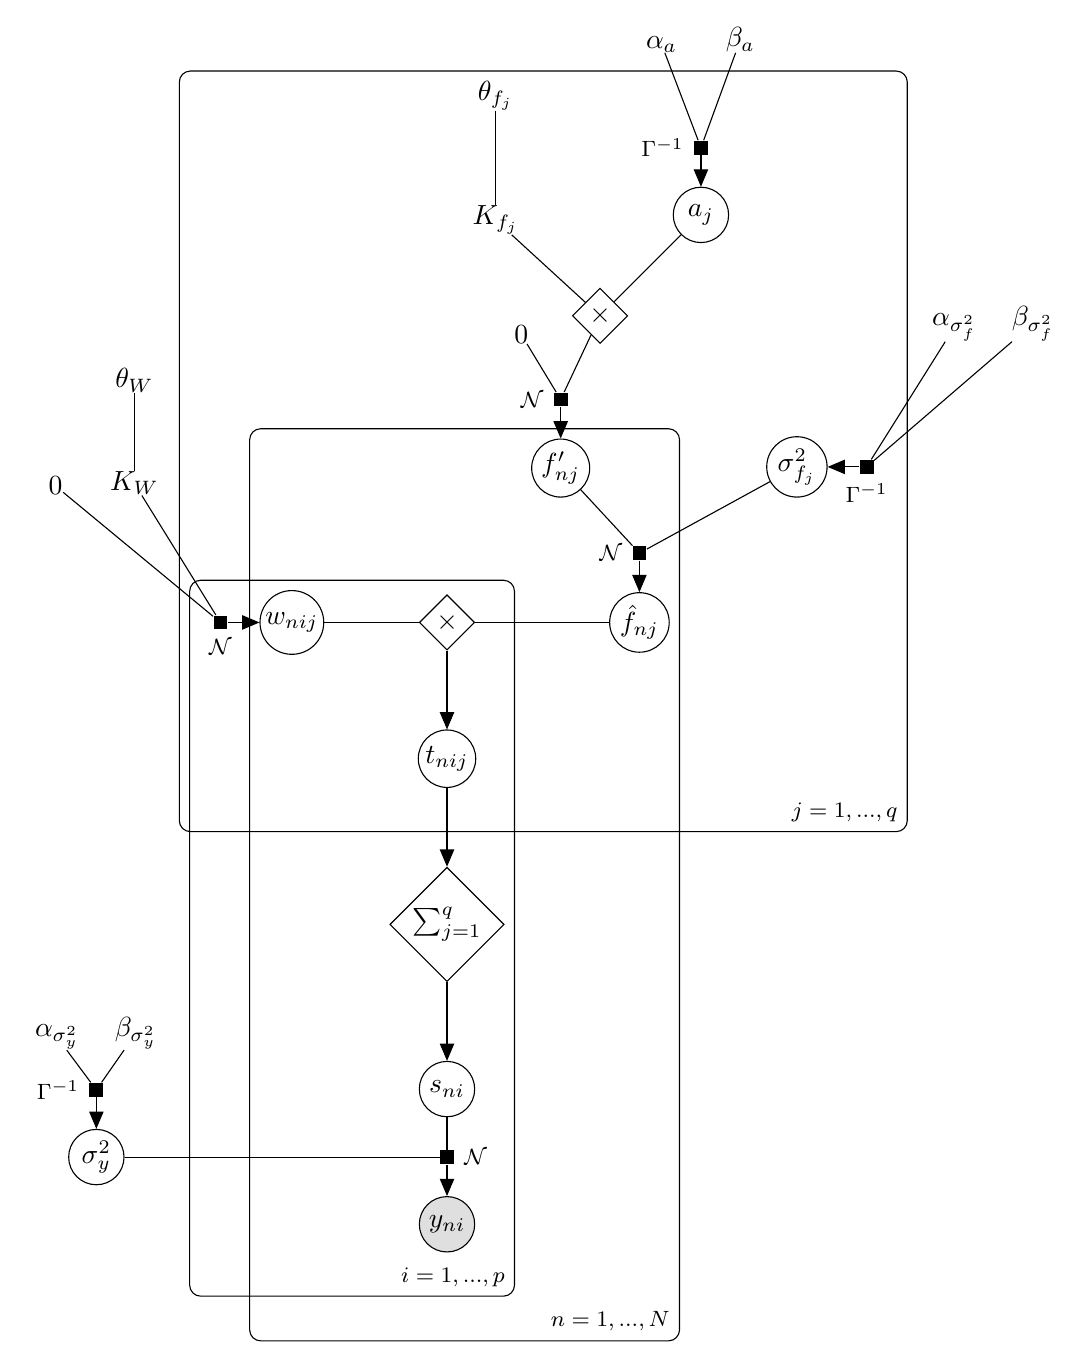
\begin{tikzpicture}

  % Define nodes

  % Y
  \node[obs]          (y)   {$y_{ni}$}; %
  \factor[above=of y] {y-f} {right:$\mathcal{N}$} {} {} ; %
  
  % S_{ni}
  \node[latent, above=of y] (s) {$s_{ni}$}; %
  
  % T_{nij}
  \node[det, above=of s] (sum) {$\sum_{j=1}^{q}$}; %
  \node[latent, above=of sum] (t) {$t_{nij}$};
  
  % W and f_hat
  \node[det, above=of t] (times1) {$\times$};
  \node[latent, left=1.2 of times1] (w) {$w_{nij}$};
  \node[latent, right=1.2 of times1, xshift=0.5cm] (f_hat) {$\hat{f}_{nj}$};

  % f' and sigma^2_f
  \node[latent, above=1.2 of f_hat, xshift=-1cm] (f) {$f'_{nj}$};
  \node[latent, above=1.2 of f_hat, xshift=2cm] (sigma_f) {$\sigma^2_{f_j}$};

  % W hyperparameters
  \node[const, above=1.2 of w, xshift=-3cm] (W_mean) {$0$} ; %
  \node[const, above=1.2 of w, xshift=-2cm]  (K_W) {$K_W$} ; %
  \node[const, above=of K_W] (theta_w) {$\theta_W$} ; %
  
  % sigma^2_f hyperparameters
  \node[const, above=1.2 of sigma_f, xshift=2cm] (a_f) {$\alpha_{\sigma^2_{f}}$};
  \node[const, above=1.2 of sigma_f, xshift=3cm] (b_f) {$\beta_{\sigma^2_{f}}$};
  
  % f' hyperparameters
  \node[const, above=1.2 of f, xshift=-0.5cm] (f_mean) {$0$};
  \node[det, above=1.2 of f, xshift=0.5cm] (times2) {$\times$};
  \node[const, above left=1.2 of times2] (K_f) {$K_{f_j}$};
  \node[latent, above right=1.2 of times2] (a) {$a_j$};
  \node[const, above=1.2 of K_f] (theta_f) {$\theta_{f_j}$};
  \node[const, above=1.7 of a, xshift=-0.5cm] (a_a) {$\alpha_a$};
  \node[const, above=1.7 of a, xshift=0.5cm] (b_a) {$\beta_a$};
  
  % noise
  \node[latent, left=4cm of y-f]         (sigma_y)   {$\sigma^2_y$}; %
  \node[const, above=of sigma_y, xshift=-0.5cm] (a_y)  {$\alpha_{\sigma^2_y}$} ; %
  \node[const, above=of sigma_y, xshift=0.5cm]  (b_y)  {$\beta_{\sigma^2_y}$} ; %

  % Factors
  \factor[left=of w] {w-f} {below:$\mathcal{N}$} {W_mean,K_W} {w} ; %
  \factor[above=of f_hat] {f_hat-f} {left:$\mathcal{N}$} {f,sigma_f} {f_hat} ; %
  \factor[above=of sigma_y] {sigma_y-f} {left:$\Gamma^{-1}$} {a_y,b_y} {sigma_y} ; %
  \factor[right=of sigma_f] {sigma_f-f} {below:$\Gamma^{-1}$} {a_f,b_f} {sigma_f};
  \factor[above=of f] {f-f} {left:$\mathcal{N}$} {f_mean,times2} {f};
  \factor[above=of a] {a-f} {left:$\Gamma^{-1}$} {a_a,b_a} {a};
  \factoredge {s,sigma_y} {y-f} {y} ; %

  % Edges
  \edge {sum} {s};
  \edge {t} {sum};
  \edge {times1} {t} ;
  \edge[-] {w,f_hat} {times1} ;
  \edge[-] {theta_w} {K_W};
  \edge[-] {K_f,a} {times2};
  \edge[-] {theta_f} {K_f};
  

  % Plates
  \plate {all_i} { %
    (y)(y-f)(y-f-caption) %
    (s) %
    (sum) %
    (t) %
    (times1) %
    (w)(w-f)(w-f-caption) %
  } {$i=1,...,p$} ;
  \plate {all_n} {%
    (y)(y-f)(y-f-caption) %
    (s) %
    (sum) %
    (t) %
    (times1) %
    (w) %
    (f_hat)(f_hat-f)(f_hat-f-caption) %
    (f) %
    (all_i.south east) %
    (all_i.north east)
  } {$n=1,...,N$} ;
  \plate {all_j} {%
    (t) %
    (times1) %
    (w)(w-f)(w-f-caption) %
    (f_hat)(f_hat-f)(f_hat-f-caption) %
    (sigma_f)(sigma_f-f)(sigma_f-f-caption) %
    (f)(f-f)(f-f-caption) %
    (f_mean) %
    (times2) %
    (K_f) %
    (a)(a-f)(a-f-caption) %
    (theta_f) %
    (all_i.north west)
  } {$j=1,...,q$} ;

\end{tikzpicture}
\end{document}
